\documentclass{classrep}
\usepackage[utf8]{inputenc}
\usepackage{color}
\usepackage[polish]{babel}
\usepackage[T1]{fontenc}
\usepackage{enumerate}
\usepackage{graphicx}
\usepackage{listings}
\usepackage{float}
\restylefloat{table}
\usepackage{multirow}
\usepackage[normalem]{ulem}
\useunder{\uline}{\ul}{}
\selectlanguage{polish}

\studycycle{Informatyka, studia dzienne, I st.}
\coursesemester{VI}

\coursename{Komputerowe systemy rozpoznawania}
\courseyear{2018/2019}

\courseteacher{dr hab. inż. Adam Niewiadomski}
\coursegroup{poniedziałek, 12:15}

\author{
  \studentinfo{Stanisław Zakrzewski}{210360} \and
  \studentinfo{ Maciej Socha}{210321}
}

\title{Zadanie 1: Ekstrakcja cech, miary podobieństwa, klasyfikacja}

\begin{document}
\maketitle
\newpage

\section{Cel}
Celem zadania było poznanie oraz zaimplementowanie różnych metod ekstrakcji cech z tekstów, określania podobieństwa oraz klasyfikacji tekstów.

\section{Wprowadzenie}
	Celem projektu jest stworzenie programu pozwalającego na klasyfikację  wybranego zbioru elementów. Klasyfikatorem wybranym do tego celu jest metoda k-najbliższych sąsiadów.
	
	Algorytm k najbliższych sąsiadów, nazywamy też potocznie algorytmem knn, pozwala na klasyfikację zbioru wieloelementowego według określonych etykiet. Na początku działania algorytmu k najbliższych sąsiadów określane są wektory dla każdego z elementów podlegających klasyfikacji. W naszym przypadku określanie wektorów polega na odpowiednim przetworzeniu tekstu zawierającego się w elementach zbioru do klasyfikacji. Następnie wektory są umieszczane na przestrzeni n elementowej, gdzie n stanowi liczebność elementów w wektorze. Odsłaniane są etykiety, domyślnie 10\% dla każdej z etykiet. Odsłonięcie etykiet stanowi jeden ze sposobów rozwiązania problemu zimnego startu. Następnie kolejne etykiety są nadawane kolejnym elementom, poprzez znalezienie k najbliższych elementów i wybranie spośród etykiet należących do danych elementów tych, które są najliczniejsze, w przypadku identycznej liczebności etykiet wybierana jest ta, której średnia odległość do aktualnie klasyfikowanego elementu jest mniejsza.
	
	Zaimplementowaliśmy 4 metody ekstrackji cech, będziemy je nazywać kolejno:
	\begin{itemize}
	    \item Pierwszy sposób ekstrakcji
	    \item Drugi sposób ekstrakcji
	    \item Trzeci sposób ekstrakcji
	    \item Czwarty sposób ekstrakcji
	\end{itemize}
	
	\subsection{Pierwszy sposób ekstrakcji}
	Wektor cech w pierwszym sposobie ekstrakcji jest tworzony poprzez wybieranie słów kluczowych z tekstów. Kolejno dla każdej z etykiet wykonuje się kroki:
	\begin{enumerate}
	    \item Z tekstów zawierających daną etykietę wybierane są wszystkie słowa jakie się w nich znajdują i tworzony jest z nich wektor.
	    \item Z wektora usuwane są słowa znajdujące się na stop liście.
	    \item Z wektora usuwane są jakiekolwiek liczby.
	    \item Przy pomocy pomiaru częstotliwości pojawiania się słów bliżej początku tekstu, wybierana jest określona wcześniej liczba słów.
	\end{enumerate}
	Następnie wszystkie wektory powstałe dla każdej etykiety łączone są w jeden wektor nie zawierający powtórzeń.
	Wektor cech w pierwszym sposobie ekstrakcji przyjmuje postać:
	\[ v = ["word1", "word2", ... "wordN"]\]
	Następnie dla każdego z tekstów znajdującego się w zbiorze testowym ustalany jest wektor poprzez określenie podobieństwa słów z tekstu do słów w wektorze. Następnie następuje normalizacja do przediału wartości od 0 do 1. Powstają wtedy wektory gotowe do umieszczenia w przesrzeni knn przyjmujące na przykład postać:
	\[ v=[0, 0.4, 0.6, 1, 0.6]\]
	
\subsection{Drugi sposób ekstrakcji}
	Wektor w drugim sposobie ekstrakcji składa się z 11 cech(11 liczb). Pierwsza z nich określa liczbę zdań w tekście, druga liczbę słów. Następnie 8 kolejnych liczb odpowiada: liczbie słów składających się z 2 i mniej liter, liczbę słów składających się z 3 liter, liczbę słów składających się z 4 liter, liczbę słów składających się z 5 liter, liczbę słów składających się z 6 liter, liczbę słów składających się z 7 liter, liczbę słów składających się z 8 liter oraz  liczbę słów składających się z 9 i więcej liter. Ostatnim elementem jest liczba słów zaczynających się z wieliej litery.\\
	Wektor cech w drugim sposobie ekstrakcji przyjmuje postać:
	\[v=[1, 2, 3, 5, 12, 3, 3, 4, 10, 5, 0] \]
	
\subsection{Trzeci sposób ekstrakcji}
	Trzeci sposób jest analogiczny do pierwszego, różni się tylko zamiana słów na reprezentujące je skróty. Skrót taki składa się z pierwszej litery słowa, ostatniej litery słowa i liczby liter w słowie, przykładowo przyjmiuje wartość:\\
	\[ s(american)=an8\]
	Podobnie jak w pierwszym sposobie ekstrakcji(proszę zwrócić uwagę na dodanie 4 punktu) wykonuje sie kroki:
		\begin{enumerate}
	    \item Z tekstów zawierających daną etykietę wybierane są wszystkie słowa jakie się w nich znajdują i tworzony jest z nich wektor.
	    \item Z wektora usuwane są słowa znajdujące się na stop liście.
	    \item Z wektora usuwane są jakiekolwiek liczby.
	    \item Zamiana słów na skróty.
	    \item Przy pomocy pomiaru częstotliwości pojawiania się słów bliżej początku tekstu, wybierana jest określona wcześniej liczba słów.
	\end{enumerate}
	Następnie wszystkie wektory powstałe dla każdej etykiety łączone są w jeden wektor nie zawierający powtórzeń.\\
	Wektor cech w trzecim sposobie ekstrakcji przyjmuje postać:\\
	\[ v = ["ak8", "wn6", ... "fg5"]\]
	Następnie dla każdego z tekstów znajdującego się w zbiorze testowym ustalany jest wektor poprzez określenie podobieństwa słów z tekstu do słów w wektorze. Następnie następuje normalizacja do przediału wartości od 0 do 1. Powstają wtedy wektory gotowe do umieszczenia w przesrzeni knn przyjmujące na przykład postać:\\
	\[ v=[0, 0.4, 0.6, 1, 0.6]\]
	W trzecim sposobie ekstrakcji zastosowana została własna miara podobieństwa obiczaza poprzez wzór przedstawiony w formie wycinku kodu z klasy \(OurComparator\):
	\begin{lstlisting}
if(s1.charAt(0)==s2.charAt(0) && s1.charAt(1)==s2.charAt(2)) {
    return (float)1/(1+Math.abs(Integer.parseInt(s1.substring(2))
        - Integer.parseInt(s2.substring(2))));
}
return 0;
	\end{lstlisting}
	Gdzie \(s1\) i \(s2\) są elementami, które ze sobą porównujemy.
	
	
	\subsection{Czwarty sposób ekstrakcji}
	Wektor w czwartym sposobie ekstrakcji składa się z 6 elementów. Pierwsze 4 są generowane poprzez podzielenie liczby różnych końcówek słów znajdujących się na końcu linii(kolejno w w 1 liczbie końcówka składa się z 1 litery w 2 z 2 liter w 3 z 3 liter a w 4 z 4 liter) poprzez liczbę linijek. Piąty element stanowi maksymalną różnicę w liczbie sylab pomiędzy linijkami, podzieloną poprzez maksymalną liczbę sylab w jednej linijce. Ostatą wartość tworzy się poprzez podzielenie maksymalnej różnicy długości w literach linijek w tekście, poprzez maksymalną liczbę liter w linijce.
	Wektor cech w czwartym sposobie ekstrakcji przyjmuje postać:
	\[ v=[0.1, 0.3, 0.5, 0.1, 0.8, 0.5]\]
	
	\subsection{Pozostałe wzory użyte w programie}
	
	Obliczenia odległości dokonano w trzech metrykach.
	
	Pierwszą z nich jest metryka Euklidesa, odległość \( d \) obliczana jest przy pomocy wzoru, gdzie \(n\) oznacza długość wektora w przestrzeni knn: 
\[ d\left ( x,y \right )=\sqrt{\left ( x_{1}-y_{1} \right )^{2} + \left ( x_{2}-y_{2} \right )^{2} + ... + \left ( x_{n}-y_{n} \right )^{2}} \]

	Drugą z nich jest metryka Manhattana, nazywana również metryką uliczną, taksówkarską lub miejską. Odległość jest obliczana przy pomocy wzoru:
\[ d\left ( x,y \right )=\sum|x_{i}-y_{i}| \]

	Trzecią i zarazem ostatnią jest metryka Czebyszewa, odległość jest obliczana przy pomocy wzoru:
$$ d(x,y) = max_{i}   |x_{i}-y_{i}| $$

	Podobieństwo pomiędzy poszczególnymi słowami wyznaczaliśmy przy pomocy dwóch spobów:
Pierwszym z nich była uogólniona miara n-gramów. Obliczana jest przy pomocy wzoru:

$$ \mu_{N}(s_{1}, s_{2})= \frac{2}{N^{2} + N}  \sum_{i=1}^{N(s_{1})} \sum_{j=1}^{N(s_{1})-i+1}  h(i,j) $$

Drugim były natomiast trigramy. Ich użycie miało na celu pokazanie przewagi uogólnionej miary n-gramów nad miarą z jednym jasno określonym n. Obliczaja jest przy pomocy wzoru:

$$ sim_{n}(s_{1}, s_{2}) = \frac{1}{N - n + 1} \sum_{i = 1}^{N-n+1} h(i) $$

\section{Opis implementacji}
Algorytmy zostały zaimplementowane w języku Java w wersji 11. Dodatkowo na potrzemy procesu lemmatyzacji wykorzystano, udostępnioną przez Stanford Natural Language Processing Group, biliotekę CoreNLP w wersji 3.9.2. Biblioteka ta jest udostępniona z licencją GNU General Public License v3 co pozwala nam korzystać z niej w naszym programie. Biblioteka ta jest bardzo obszerna, w naszym programie wykorzystujemy jedynie funkcjonalność lemmatyzacji. Jest ona zaimplementowana w klasie StanfordLemmatizer. Implementacja tej klasy została bezpośrednio zaczerpnięta z dokumentacji[5]. Poniżej przedstawiono uproszczony diagram klas. Zaznaczone zostały na nim kluczowe dla działania naszego programu klasy.\\

\begin{figure}[ht]
	\makebox[\linewidth]{
		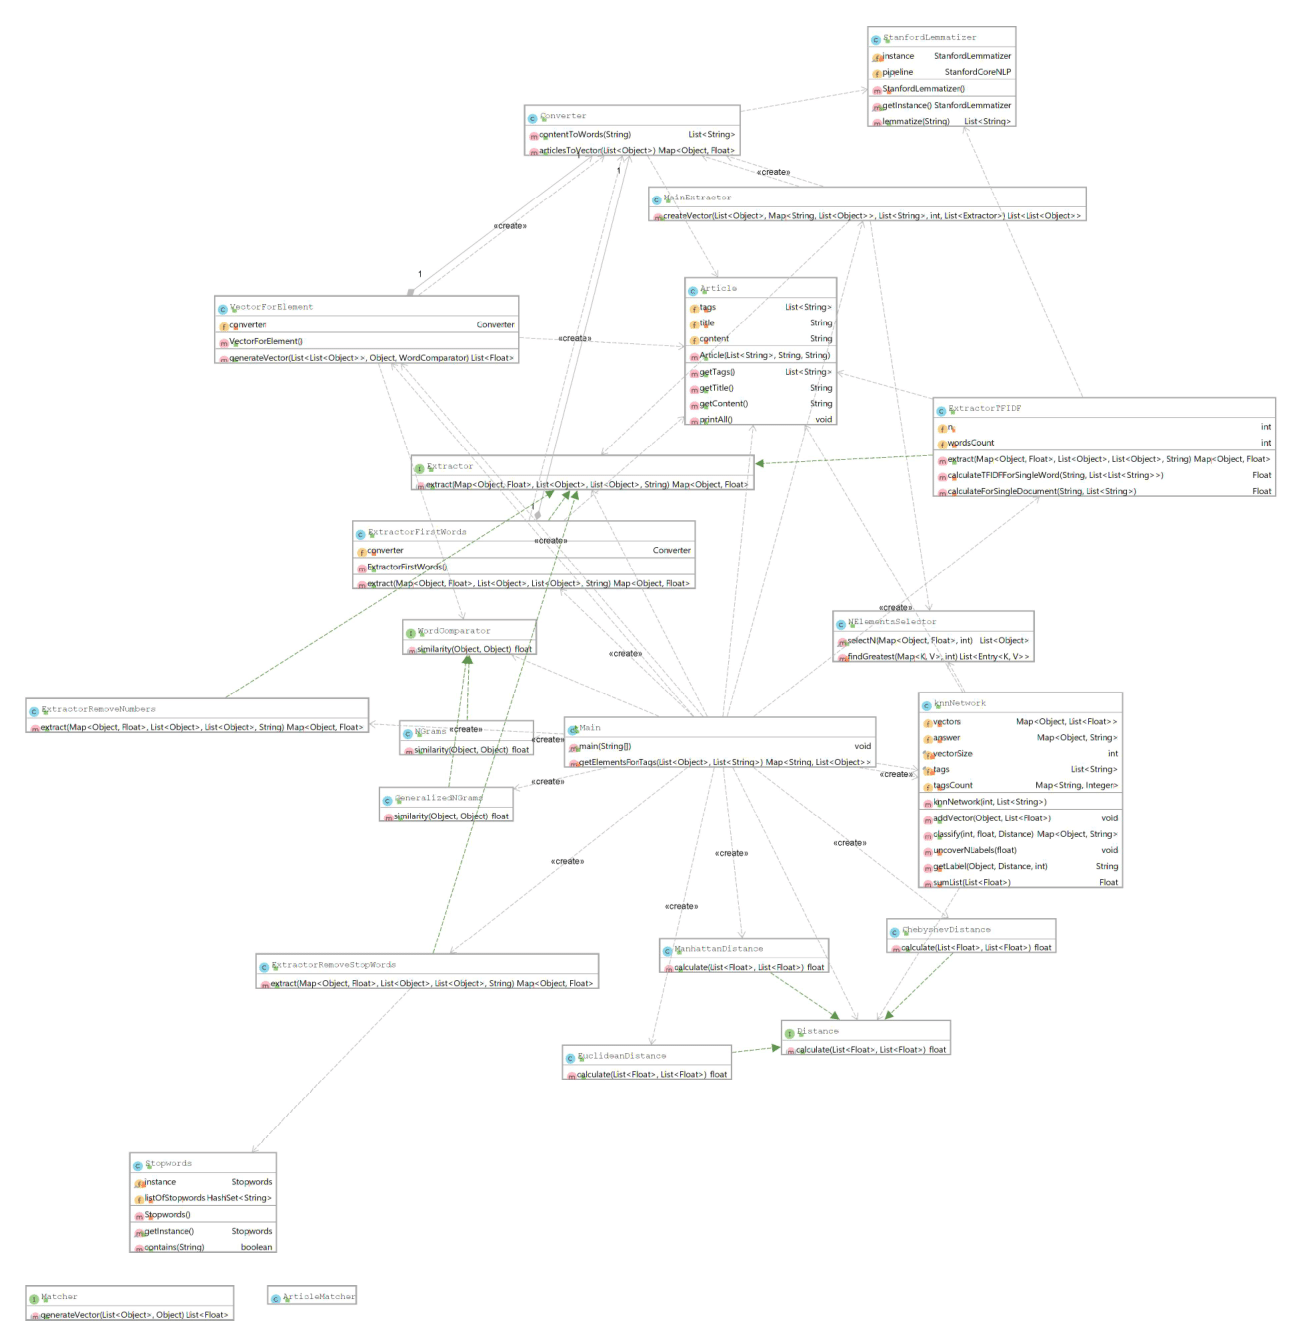
\includegraphics[scale=0.4]{uml.png}
	}
	\caption{UML Diagram}
\end{figure}

Klasa Article odpowiada za przechowywanie informacji niezbędnych do działania programu. Wykorzystujemy ją zarówno do przetwarzania artukułów zawartych w zbiorze danych reuters jak i zestawu artykułów przygotowanego przez nas samych.\\
Interfejs Extractor służy i znajdująca się w nim metoda extract jest wykorzystywana przy procesie ekstakcji cech. Implementują ją liczne klasy zawierające sie w dwóch sposobach ekstarakcji cech zawartych w programie.\\
Klasa knnNetwork zawiera w sobie implementację algorytmu k najbliższych sąsiadów do ustalania przynależności wektorów odpowiadającycm przekazanym do programu elementom. Klasa pozwala na dodawanie wektorów wraz z odpowiadającymi im elementami, a następnie klasyfikowanie ich przy przekazaniu odpowiedniego parametru k oznaczającego liczbę sąsiadów, uncoveredLabelFraction zapomocą którego przekazujemy jaka część tekstów będzie miała odkryte etykiety oraz distance, metrykę obliczania dystansu pomiędzy wektorami.\\
Pakiet calculatedistance zawiera w sobie interfejs Distance oraz implementujące go klasy ChebyshevDistance(metryka Czebyszewa), EuclideanDistance(metryka Euklidesa) oraz ManhattanDistance(metryka uliczna). Są to wymagane przez treść zadania metryki pomiaru odległości pomiędzy wektorami.\\
Za przekazywanie danych do programu odpowiada plik config.txt zawierający w sobie wszystkie potrzebne do działania programu parametry. Są to odpowiednio:
\begin{itemize}
	\item tagClass - tag dla którego etykiety będzie nadawał program
	\item folderPath - ścieżka do folderu z plikami z danymi
	\item articlesToReadCount - liczba plików z artykułami, które program ma wczytać
	\item k - liczba najbliższych sąsiadów według których algorytm będzie klasyfikował
	\item fractionOfUncoveredForEachTag - część elementów należących do każdej z etykiet, która ma zostać odkryta w klasyfikacji knn
	\item tags - etykiety, według których program ma klasyfikować
	\item numberOfElementsPerTag - liczba elementów jakie ma zawierać w sobie cecha dla każdej z etykiet
	\item trainToTestRatio - stosunek zbioru treningowego do testowego
	\item distanceKNN - metryka pomiaru dystansu w przestrzeni dla algorytmu knn
	\item wordSimilarity - metryka podobieństwa słów
	\item extractors - zestaw ekstraktorów
\end{itemize}
\newpage

\section{Materiały i metody}
Klasyfikacja tekstów Reutersa oraz danych zebranych przez nas została wykonana dla obu sposobów ekstrakcji cech i dla każdej z 3 metryk obliczania dystansu w algorytmie k najbliższych sąsiadów. Dla parametru k wybrano niektóre wartości ze zbioru (3, 5, 8, 13, 21), tak aby jak najlepiej ukazać właściwości każdego z sposobów ekstrakcji oraz najlepiej dopasować je do zbioru danych testowych. Klasyfikacja na zbiorze Reutersa według tagu PLACES została przeprowadzona dla sześciu etykiet (west-germany, usa, uk, canada, france, japan)(13766 elementów), przy stosunku zbioru treningowego do testowego 60\%(8260 elementów) do 40\%(5506 elementów) i dla 10\%(551 elementów) odkrytych etykiet w zbiorze testowym. W drugim przypadku według tagu TOPICS etykietowano przy pomocy dwóch etykiet (coffee i gold), przy równym podziale na zbiór treningowy i testowy. Natomiast w naszych tekstach klasyfikacja nastąpiła według tagu REVIEWS dla dwóch etykiet (movie, restaurant), równego podziału zbioru elementów na część treningową i testową oraz 20\%(10 etykiet) odkrytych etykiet w zbiorze testowym. Dodatkowo do przetestowania czwartego sposobu ektrakcji użyto zbioru własnego składającego się w połowie z wierszy Williama Blake'a a w połowie z artykułów Reutera, jego liczebnośc wynosi 100 elementów, jest on podzielony na dwie części treningową i testową z czego w testowej odkryte jest 20\% etykiet(10 etykiet).

Do zbadania wyników klasyfikacji posłużyliśmy metodą tablicy pomyłek (zwaną również macierzą błędów, ang. confusin matrix). Pozwala ona ocenić jakoś klasyfikacji. Poniżej znajduje się tabela wyjaśniająca sposób jej tworzenia.
\begin{table}[H]
\begin{tabular}{|c|c|c|}
\hline
Klasa rzeczywista & Klasyfikacja jako Pozytywna                                                             & Klasyfikacja jako Negatywna                                                              \\ \hline \hline
Pozytywna         & \begin{tabular}[c]{@{}c@{}}Prawdziwie Pozytywna\\ (ang. True Positive, TP)\end{tabular} & \begin{tabular}[c]{@{}c@{}}Fałszywie Negatywna\\ (ang. False Negative, FN)\end{tabular}   \\ \hline
Negatywna         & \begin{tabular}[c]{@{}c@{}}Fałszywie Pozytywna\\ (ang. False Positive, FP)\end{tabular} & \begin{tabular}[c]{@{}c@{}}Prawdziwie Negatywna\\ (ang. True Negative, TN)\end{tabular} \\ \hline
\end{tabular}
\caption{Macierz błędów}
\end{table}
Skrótów angielskich nazw będziemy używać dalej przy określaniu miar. Znając te wartości jesteśmy w stanie obliczyć kolejne miary:
\begin{enumerate}
	\item Accuracy
	\item Precision
	\item Recall (Sensitivity)
\end{enumerate}
opisane poniżej.
\newpage
\subsection{Accuracy}
Dokładność (ang. Accuracy) jest ogólną efektywnością klasyfikacji. Wyraża się wzorem:
$$ Accuracy = \frac{tp+tn}{tp+fn+fp+tn} $$

\subsection{Precision}
Precyzja (ang. Precision) oznacza zgodność etykiet z pozytywnie zaklasyfikowanymi cechami.
$$ Precision = \frac{tp}{tp+fp} $$

\subsection{Recall}
Czułość (ang. Recall lub Sensitivity) jest to stosunek poprawnie zaklasyfikowanych pozytywnych przypadków do liczby pozytywnych przyadków w zbiorze
$$ Recall = \frac{tp}{tp+fn} $$

\section{Wyniki}
Wyniki kolejnych przeprowadzanych eksperymentów zostały umieszczone poniżej.
\subsection{Wyniki klasyfikacji dla tagu PLACES}
Wyniki eksperymentów dla tagu PLACES zostały przedstawione w tabeli~\ref{tab:PLACES1} oraz na rysunkach od~\ref{fig:PLACES1} do~\ref{fig:PLACES4}.\\
\begin{table}[H]
\begin{tabular}{|l|l|l|l|l|l|l|}
\hline
             & west-germany & usa  & uk  & france & canada & japan \\ \hline
west-germany & 59           & 99   & 2   & 5      & 0      & 4     \\ \hline
usa          & 6            & 5334 & 47  & 21     & 26     & 39    \\ \hline
uk           & 1            & 275  & 156 & 8      & 9      & 7     \\ \hline
france       & 0            & 26   & 3   & 90     & 0      & 7     \\ \hline
canada       & 0            & 252  & 7   & 1      & 165    & 1     \\ \hline
japan        & 0            & 71   & 2   & 1      & 1      & 159   \\ \hline
\label{tab:PLACES1}
\caption{Confusion Matrix dla tagu PLACES i etykiet: west-germany, usa, uk, france, canada, japan.}
\end{tabular}
\end{table}
\begin{figure}[H]
  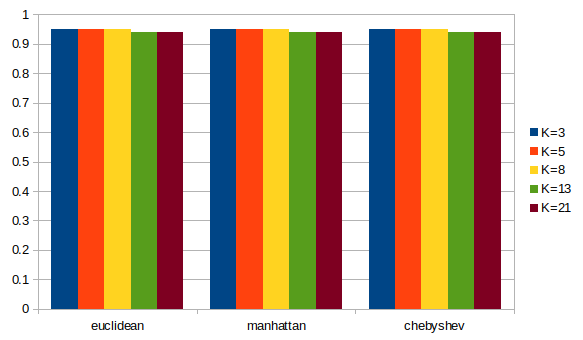
\includegraphics[width=\linewidth]{wykresy/1ext5k3mp_mcacc.png}
  \caption{Dane przedstawiające wartość parametru Multi-Class Accuracy dla wybranych wartości k i trzech zawartych w programie metryk.}
  \label{fig:PLACES1}
\end{figure}
\begin{figure}[H]
  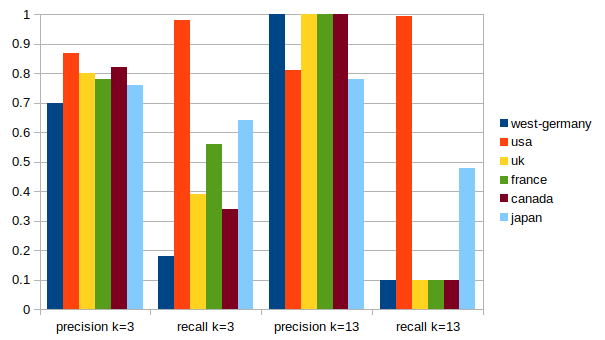
\includegraphics[width=\linewidth]{wykresy/1ext2k6tag_precrec.png}
  \caption{Wyniki ekstrakcji pierwszym ekstraktorem przedstawione poprzez wartości parametrów precision i recall dla dwóch wartości k(3 oraz 13) dla sześciu etykiet(west-germany, usa, uk, france, canada, japan).}
  \label{fig:PLACES2}
\end{figure}
\begin{figure}[H]
  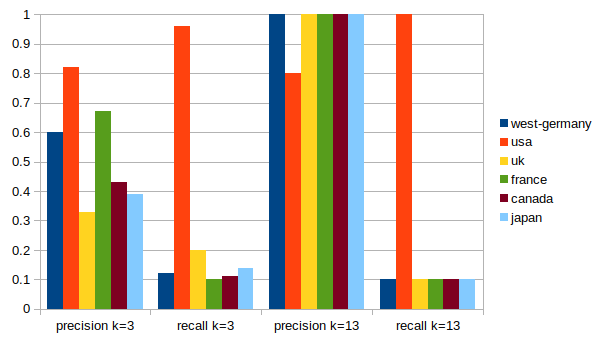
\includegraphics[width=\linewidth]{wykresy/2ext2k6tag_precrec.png}
  \caption{Wyniki ekstrakcji drugim ekstraktorem przedstawione poprzez wartości parametrów precision i recall dla dwóch wartości k(3 oraz 13) dla sześciu etykiet(west-germany, usa, uk, france, canada, japan).}
  \label{fig:PLACES3}
\end{figure}
\begin{figure}[H]
  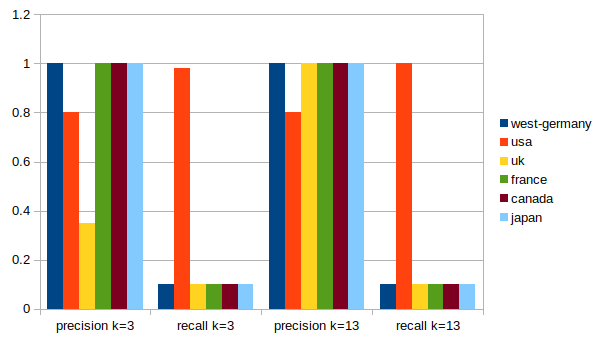
\includegraphics[width=\linewidth]{wykresy/3ext2k6tah_precrec.png}
  \caption{Wyniki ekstrakcji trzecim ekstraktorem przedstawione poprzez wartości parametrów precision i recall dla dwóch wartości k(3 oraz 13) dla sześciu etykiet(west-germany, usa, uk, france, canada, japan).}
  \label{fig:PLACES4}
\end{figure}
\newpage
\subsection{Wyniki klasyfikacji dla tagu TOPICS}
Wyniki eksperymentów dla tagu TOPICS zostały przedstawione na rysunkach od~\ref{fig:TOPICS1} do~\ref{fig:TOPICS3}.\\
\begin{figure}[H]
  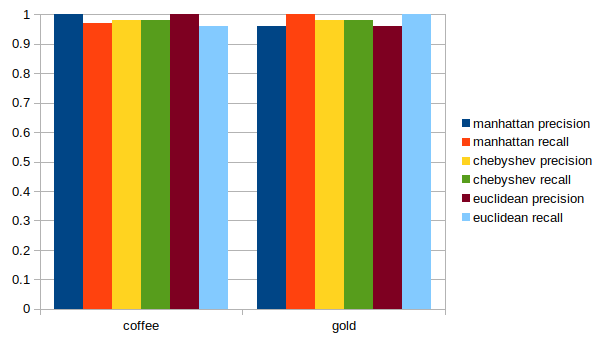
\includegraphics[width=\linewidth]{wykresy/1ext2tag3mp_precrec.png}
  \caption{Wyniki ekstrakcji pierwszym ekstraktorem przedstawione przy poprzez wartości precision i recall dla trzech różnych metryk(manhattana, czebyszewa i euklidesa) dla dwóch etykiet(coffee, gold).}
  \label{fig:TOPICS1}
\end{figure}
\begin{figure}[H]
  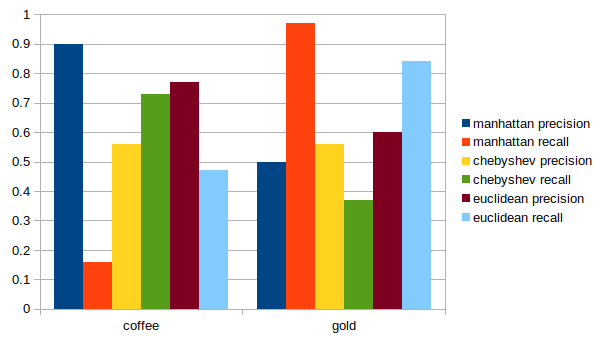
\includegraphics[width=\linewidth]{wykresy/2ext2tag3mp_precrec.png}
  \caption{Wyniki ekstrakcji drugim ekstraktorem przedstawione przy poprzez wartości precision i recall dla trzech różnych metryk(manhattana, czebyszewa i euklidesa) dla dwóch etykiet(coffee, gold).}
  \label{fig:TOPICS2}
\end{figure}
\begin{figure}[H]
  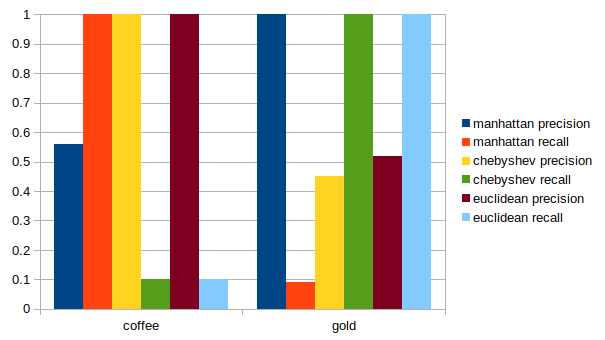
\includegraphics[width=\linewidth]{wykresy/3ext2tag3mp_precrec.png}
  \caption{Wyniki ekstrakcji trzecim ekstraktorem przedstawione przy poprzez wartości precision i recall dla trzech różnych metryk(manhattana, czebyszewa i euklidesa) dla dwóch etykiet(coffee, gold).}
  \label{fig:TOPICS3}
\end{figure}

\subsection{Wyniki klasyfikacji dla tagu REVIEWS}
Wyniki eksperymentów dla tagu REVIEWS zostały przedstawione na rysunkach~\ref{fig:REVIEWS1} i~\ref{fig:REVIEWS2}.\\
\begin{figure}[H]
  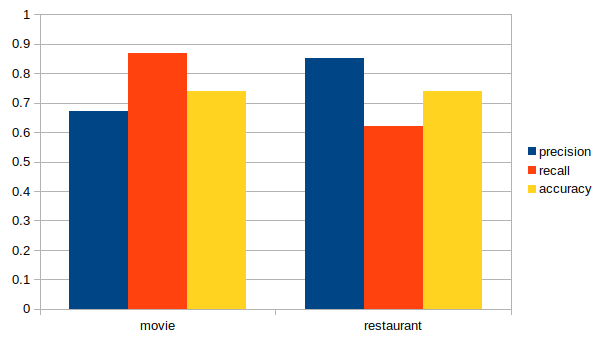
\includegraphics[width=\linewidth]{wykresy/1ext2tagNG_precrecacc.png}
  \caption{Wyniki ekstrakcji pierwszym ekstraktorem przedstawione poprzez wartości parametrów precision, recall i accuracy dla miary podobieństwa trigramów dla dwóch etykiet(movie, restaurant).}
  \label{fig:REVIEWS1}
\end{figure}
\newpage
\begin{figure}[H]
  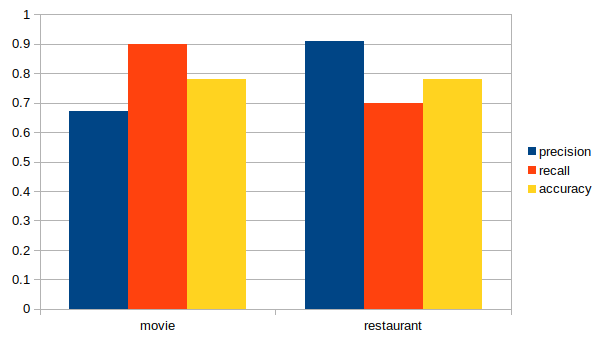
\includegraphics[width=\linewidth]{wykresy/2ext2tagGNG_precrecall.png}
  \caption{Wyniki ekstrakcji pierwszym ekstraktorem przedstawione poprzez wartości parametrów precision, recall i accuracy dla miary podobieństwa uogólnionej miary n-gramów dla dwóch etykiet(movie, restaurant).}
  \label{fig:REVIEWS2}
\end{figure}

\subsection{Wyniki klasyfikacji dla tagu LITERATURE}
Wyniki eksperymentów dla tagu LITERATURE zostały przedstawione na rysunkach~\ref{fig:LITERATURE1} i~\ref{fig:LITERATURE2}.\\
\begin{figure}[H]
  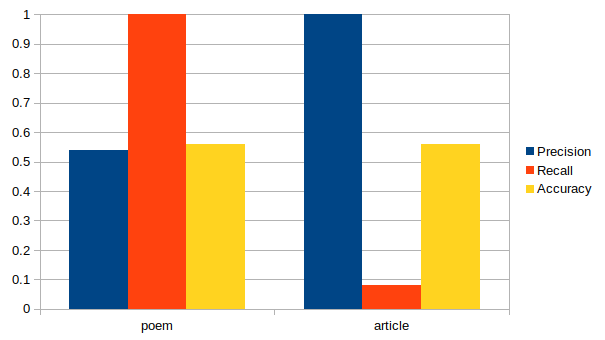
\includegraphics[width=\linewidth]{wykresy/1ext2tag_precrecacc.png}
  \caption{Wyniki ekstrakcji pierwszym ekstraktorem przedstawione poprzez wartości precision, recall i accuracy dla dwóch etykiet(poem, article).}
  \label{fig:LITERATURE1}
\end{figure}
\begin{figure}[H]
  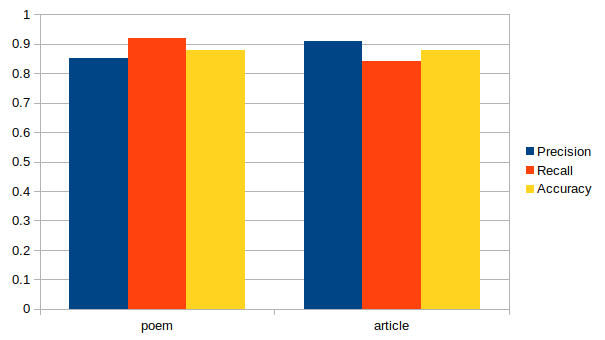
\includegraphics[width=\linewidth]{wykresy/4ext2tag_precrecacc.png}
  \caption{Wyniki ekstrakcji czwartym ekstraktorem przedstawione poprzez wartości precision, recall i accuracy dla dwóch etykiet(poem, article).}
  \label{fig:LITERATURE2}
\end{figure}
\newpage

\section{Dyskusja}
\subsection{Uwagi ogólne}
	Napisanie programu klasyfikującego uświadomiło nam, że w rozpoznawaniu danego tekstu nie liczą się jedynie znaczenia poszczególnych słów. Pozytywny wpływ na jakość klasyfikacji miało wykorzystanie w pierwszym ekstraktorze cech wybierania słów kluczowych poprzez preferowanie tych znajdujących się bliżej początku tekstu. Właściwość ta jest związana z podstawowymi założeniami artykułu prasowego, i w tekstach opracowanych przez nas recenzji, które mają na celu w pierwszych słowach określić kontekst danego tekstu. Zdajemy sobie sprawę, że dla innego typu tekstu pisanego, takiego jak na przykład opowiadanie cecha ta niekoniecznie będzie obecna, nastąpi wtedy konieczność stworzenia nowego modelu ekstrakcji cech, do którego przyjęcia nasz program jest zdolny.
	
	Bardzo ważne, przy tworzeniu programów do klasyfikacji tekstów jest rozróżnienie cech językowych od cech metajęzykowych. Poprzez cechy językowe rozumiemy cechy odnoszące się do semantyki. Semantyką nazywamy naukę o budowie wyrazów. Poprzez cechy metajęzykowe rozumiemy wszystkie cechy abstrahujące od znaczenia słów, a skupiające się na ich ułożeniu, długości, rymach, czy liczbie sylab. W pierwszym i trzecim sposobie ekstrakcji użyliśmy zarówno cech językowych jak i metajęzykowych. Natomiast w drugim sposobie użyliśmy wyłącznie cech metajęzykowych.
	
	Znacząco większa liczebność artykułów z etykietą usa negatywnie wpływa na klasyfikację klas z etykietami: west-germany, uk, france, canada i japan. Jest to szczególnie widoczne w tabeli~\ref{tab:PLACES1} przedstawiającej confusion matrix. Dodatkowo w przypadku znacznej przewagi liczebnej jednej z etykiet przydatność parametru accuracy spada, co widać na rysunku~\ref{fig:PLACES1}.
	
	Rezultaty dla przygotowywanych przez nas tekstów(Rysunki:~\ref{fig:REVIEWS1},~\ref{fig:REVIEWS2}) były znacząco niższe niż dla tekstów zaczerpniętych z bazy Reutera(Rysunki:~\ref{fig:TOPICS1},~\ref{fig:TOPICS2},~\ref{fig:TOPICS3}). Jest to zapewnie spowodowane spójnym stylem i określoną formą tekstów Reutera, podczas gdy przygotowane przez nas teksty znacząco się różniły pod względem stylistycznym jak i formalnym.
	
\subsection{Wyższość pierwszego sposobu ekstrakcji nad drugim i trzecim.}
    Zauważyliśmy znaczącą różnicę pomiędzy wartościami współczynnikow precision, recall i accuracy pomiędzy pierwszym(Rysunek~\ref{fig:PLACES2}) a drugim(Rysunek~\ref{fig:PLACES3}) i trzecim(Rysunek~\ref{fig:PLACES4}) sposobem ekstrakcji na korzyść pierwszego sposobu ekstrakcji.
    
    Wyniki lepsze niż drugi sposób ekstrakcji, sposób pierwszy osiągnął dzięki użyciu w nim cech zarówno językowych jak i metajęzykowych.
    
    Niestety nasza próba uproszczenia sposobu zapisu słów kluczowych w trzecim sposobie ekstrakcji okazała się nietrafiona. Sposób w jaki postanowiliśmy zapisać słowa kluczowe całkowicie nie jest wystarczający, aby przechować wystarzającą informację.
    
\subsection{Zrozumienie idei czwartego sposobu ekstrakcji.}
    Jak już zostało napisane powyżej w ekstrakcji cech z tekstów ważne jest aby odróżniac cechy języka od cech metajęzyka. Rozróżnienie to jest kluczowe zwłaszcza przy próbie zrozumienia dlaczego czwarty ektraktor działa tak dobrze.
    
    W czwartym ekstraktorze wykorzystane zostały cechy struktury lirycznej jaką jest wiersz(eng. poem). Są to rymy o różnej, acz rozsądnej długości, stała, bądź bardzo zbliżona do siebie liczba sylab w kolejnych linijkach oraz mała różnica w długości linijek. Dla odmiany artykuły nie zawierają w sobie żadnej z wyżej wymienionych cech. Posłużyliśmy się zatem cechami metajęzykowymi.
    
    Dla porównania cechy języka, przy pomocy których operuje najskuteczniejszy w eksperymentach na tagach PLACES, TOPICS oraz REVIEWS pierwszy ekstraktor, nie dają specjalnie wysokich wyników w przypadku tekstów z tagu LITERATURE(Rysunek~\ref{fig:LITERATURE1}) w porównaniu do wyników czwartego ekstraktora(Rysunek~\ref{fig:LITERATURE2}). Jest to spowodowane ich różnorodnością i brakiem wspólnego znaczenia semantycznego.
    
\section{Wnioski}
	Stworzenie systemu ekstrakcji cech dla danego rodzaju bądź zbioru tekstów jest zadaniem o wiele trudniejszym niż przypuszczaliśmy i wymaga nie tylko wiedzy o słowach jakie mogą się znaleźć w danym tekście, ale i dogłębnej wiedzy o wybranym typie tekstu, jak w naszym przypadku artykule jak i w wybranym przez nas, podobnej jeśli chodzi o cechy recenzji.
	
	Algorytm k najbliższych sąsiadów ma problem, w momencie, kiedy jedna z etykiet ma znacząco więcej przyporządkowanych do niej elementów. Ważne jest wtedy aby odpowiednio dobrać wartość k aby nie była zbyt wysoka. Należy też wtedy zadbać o to, aby do zbioru początkowo odkrytych etykiet dla elementów trafiły etykiety każdego rodzaju.
	
	Najlepiej radzą sobie algorytmy korzystające zarówno z cech językowych jak i metajęzykowych.

\begin{thebibliography}{0}
  \bibitem{article1} David D. Lewis.
  	\textsl{Feature Selection and Feature Extract ion for Text Categorization}, University of Chicago,\\
  	Dostępny w Internecie: \url {https://aclweb.org/anthology/H92-1041?fbclid=IwAR248ftiyFqXrFpi51IDLorT7Ngso369BPTOaOeSYE3QGG1gYD9TNfy58qc}

  \bibitem{article2} David Dolan Lewis.
  	\textsl{Representation and learning in information retrieval}, University of Massachusetts,\\
  	Dostępny w Internecie: \url {http://ciir.cs.umass.edu/pubfiles/UM-CS-1991-093.pdf}

  \bibitem{article3} David D. Lewis.
  	\textsl{Data Extraction as Text Categorization : An
Experiment With the MUC-3 Corpus}, University of Chicago,\\
	Dostępny w Internecie: \url {https://www.aclweb.org/anthology/M91-1035}

  \bibitem{article4} Marina Sokolova, Guy Lapalme.
  	\textsl{A systematic analysis of performance measures for classification tasks}, Information Processing and Management no 45,\\
  	Dostępny w internecie: \url {http://rali.iro.umontreal.ca/rali/sites/default/files/publis/SokolovaLapalme-JIPM09.pdf?fbclid=IwAR2M7_a4QxL_F4yCOB_Akp4ghkoUKrBnHT9xzCfuTcoVrLBe3lN3kIlPt00}

  \bibitem{stanford} Dokumentacja Stanford CoreNLP
    \url {https://stanfordnlp.github.io/CoreNLP}
    
  \bibitem{notatki} Adam Niewiadomski.
  	\textsl{Materiały, przykłady i ćwiczenia do przedmiotu
Komputerowe Systemy Rozpoznawania}, 21 września 2009.\\

\end{thebibliography}
\end{document}
